
In the final state, there are four jets, one charged lepton and \MET.
Various selections cuts are applied to ensure the resulting events to have 
this topology. Cut-flow plots after various selection cuts are shown in 
Figure~\ref{fig:cutflow}. Below we list out various selection requirements applied.
\begin{enumerate}
\item{\bf{Event filter and trigger}}:
    The events are passed to the filters and triggers, as discussed in 
    Section (\ref{s:secFilters}). The lepton trigger is used to enrich events 
    with lepton and significantly reduces QCD compared to other SM background.
    The number of events surviving trigger cuts for signal, background MC and 
    data are shown in the 2nd column of Tables~\ref{tab:cutflow_mu}, 
    \ref{tab:cutflow_ele}, \ref{tab:cutflow_mu_sig} and \ref{tab:cutflow_ele_sig}. 
\item {\bf{Lepton selection}}:
The event topology has only one lepton thus events having a second loose lepton 
are not selected. The lepton-veto selection for the \mujets and \ejets
channel are listed in Tables~\ref{tab:muonSel} and \ref{tab:eleSel}.
For the \mujets (\ejets) channel there cannot be any electron (muon) 
in an event. Those events where there is any electron (muon) in the \mujets (\ejets) channel are rejected. Lepton scale factors as described in Sec.~\ref{s:lepton_sf} are applied to MC events. The relative isolation cut for 
muon and electron is $I_{\rm rel}^{\mu} < 0.15$ and $I_{\rm rel}^{ele} < 0.08$, respectively. Event yields after one lepton selection are shown in the 3rd 
column of Tables~\ref{tab:cutflow_mu}, \ref{tab:cutflow_ele}, 
\ref{tab:cutflow_mu_sig} and \ref{tab:cutflow_ele_sig}.

\item {\bf{Jet selection}}:
There should be at least four jets in an event.
Jet selection cuts are listed in Table~\ref{tab:jetSel}.
The jet energy is corrected using JES and JER scale factors.
After correcting jet energy, the selections on jet as shown in 
Table~\ref{tab:jetSel} are applied. Number of events after jet selection are 
shown in the 4th column of Tables~\ref{tab:cutflow_mu},
\ref{tab:cutflow_ele}, \ref{tab:cutflow_mu_sig} and \ref{tab:cutflow_ele_sig}.

\item {\bf{\MET selection}}:
The \MET should be greater than 20 GeV. Event yields after \MET selection are 
shown in the 5th column of Tables~\ref{tab:cutflow_mu},
\ref{tab:cutflow_ele}, \ref{tab:cutflow_mu_sig} and \ref{tab:cutflow_ele_sig}.
After applying \MET selection QCD, $Z/\gamma$+jets event yields reduce more compared to \ttbar+jets, single $t$, $W$+jets, and VV processes because 
there is no genuine \MET (neutrino) at the parton level.

\item {\bf{b-jet selection}}:
For b-jet selection, the medium working point is used i.e, $b_{discr} > 0.8484$. 
The b-tag event weights, as described in Sec.~\ref{s:bTagSF}, are applied on
MC events. The events are required to have at least two b-jets.
Event yields for MC signal, background and data are shown in the 6th column of Table~\ref{tab:cutflow_mu},
\ref{tab:cutflow_ele}, \ref{tab:cutflow_mu_sig} and \ref{tab:cutflow_ele_sig}.

\item {\bf{Kinematic fit selection}}:
The kinematic fit does not converge for every event~\cite{DHondt:2006iej}.
Only those events are selected for whom the fit converges.
Also, the same cuts on kinematically fitted objects as that of reconstructed objects are used.
The direction of kinematically fitted jets should be almost same to that of the reconstructed jets.
The following kinematic fit selections are applied: 
\begin{itemize}
 \item the kinematic fit converges for selected events,
 \item $\Delta R (KF_{\rm lep}, Reco_{\rm lep}) < 0.2$,
 \item $\Delta R (KF_{\rm jets}, Reco_{\rm jets}) < 0.2$%, and
% \item $\chi^2_{kfit} >0$, $Prob_{kfit} > 0$.
\end{itemize}
Event yields after kinematic fit selections are shown in the 7th column of Tables~\ref{tab:cutflow_mu},
\ref{tab:cutflow_ele}, \ref{tab:cutflow_mu_sig} and \ref{tab:cutflow_ele_sig}.
From these tables, we see that almost half the number of events is reduced after these selections.

\item {\bf{c-jet selection}}:
The loose charm tagging working point (pfCCvsL $> -0.48$ and pfCCvsB $> -0.17$) is used to tag a jet as c-jet.
The c-tag event weights are applied following the same procedure as that for b-tag event weights.
Event yield after demanding at least 1 c-jet with the loose working point for signal, background, and data are shown in 8th column of
Tables~\ref{tab:cutflow_mu}, \ref{tab:cutflow_ele}, \ref{tab:cutflow_mu_sig} and \ref{tab:cutflow_ele_sig}.

\end{enumerate}

From Table~\ref{tab:cutflow_mu} (\ref{tab:cutflow_ele}) it can be seen that the $W + jets$ 
process is the dominant background upto 1-lepton selection. However, when the events are required to have $N_{jets} \geq 4$, the \ttjets 
becomes the dominant background. The \ttjets remains dominant background after
subsequent selection cuts. The QCD events are from MC QCD samples as shown in 
Table~\ref{tab:mcSample}.

The signal event yields for a different mass of charged Higgs after 
various selection cuts are shown in Table~\ref{tab:cutflow_mu_sig} (\ref{tab:cutflow_ele_sig}) 
for the muon (electron) + jets channel. It can be seen from 
Table~\ref{tab:cutflow_mu_sig} (\ref{tab:cutflow_ele_sig}) that the event yields are almost 
same upto 1-lepton selections for all masses of charged Higgs. 
However, after the $N_{jets} \geq 4$ selection, when \ttjets becomes the dominant 
background as shown in Table~\ref{tab:cutflow_mu} (\ref{tab:cutflow_ele}), the event yield 
for higher masses of the charged Higgs are reduced more compared to the lower masses. The 
event yield reduces because of the less phase space available between top-quark and charged 
Higgs for higher masses.
    
\begin{figure}
\centering
\subfigure[Event yields for the \mujets
channel]{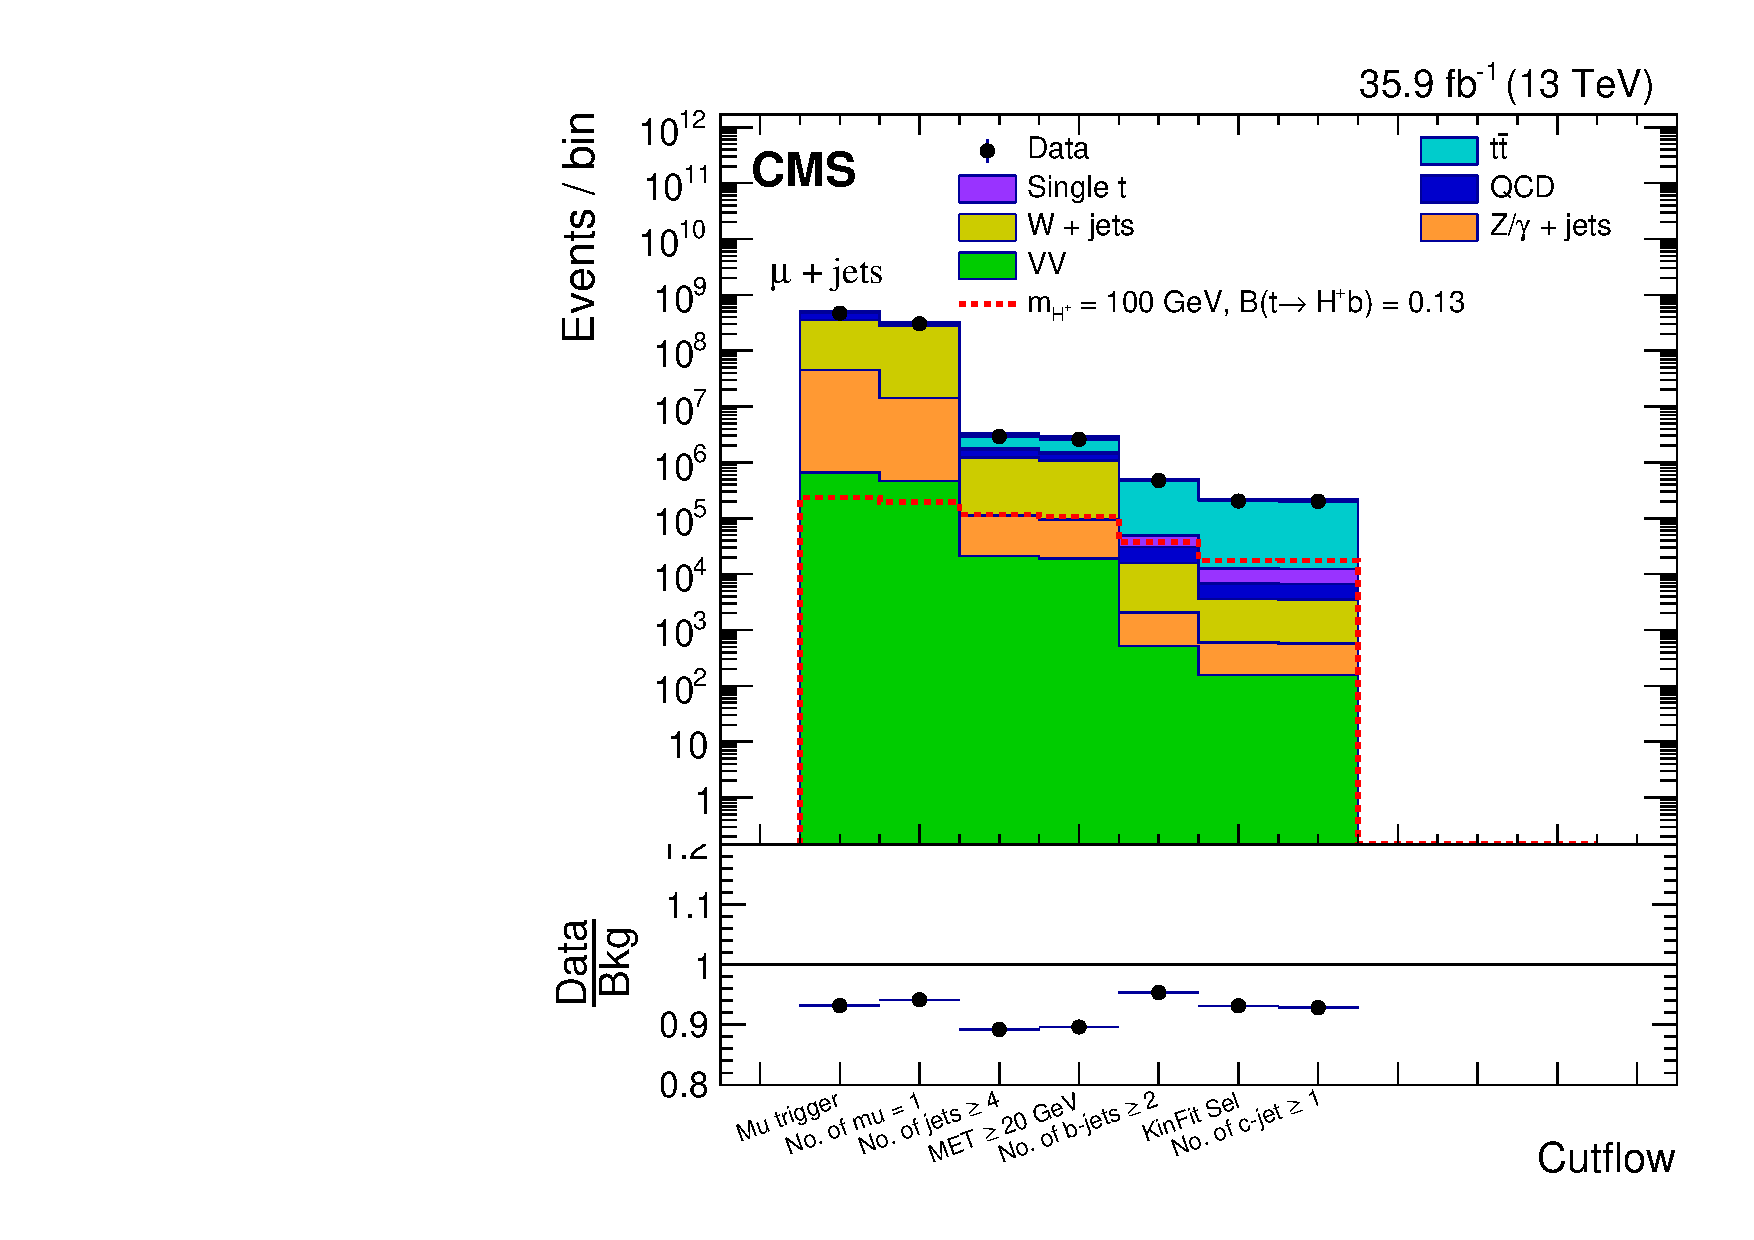
\includegraphics[width=0.50\linewidth]{Image/Muon/cutflow_mu.pdf}}
\subfigure[Event yields the \ejets
channel]{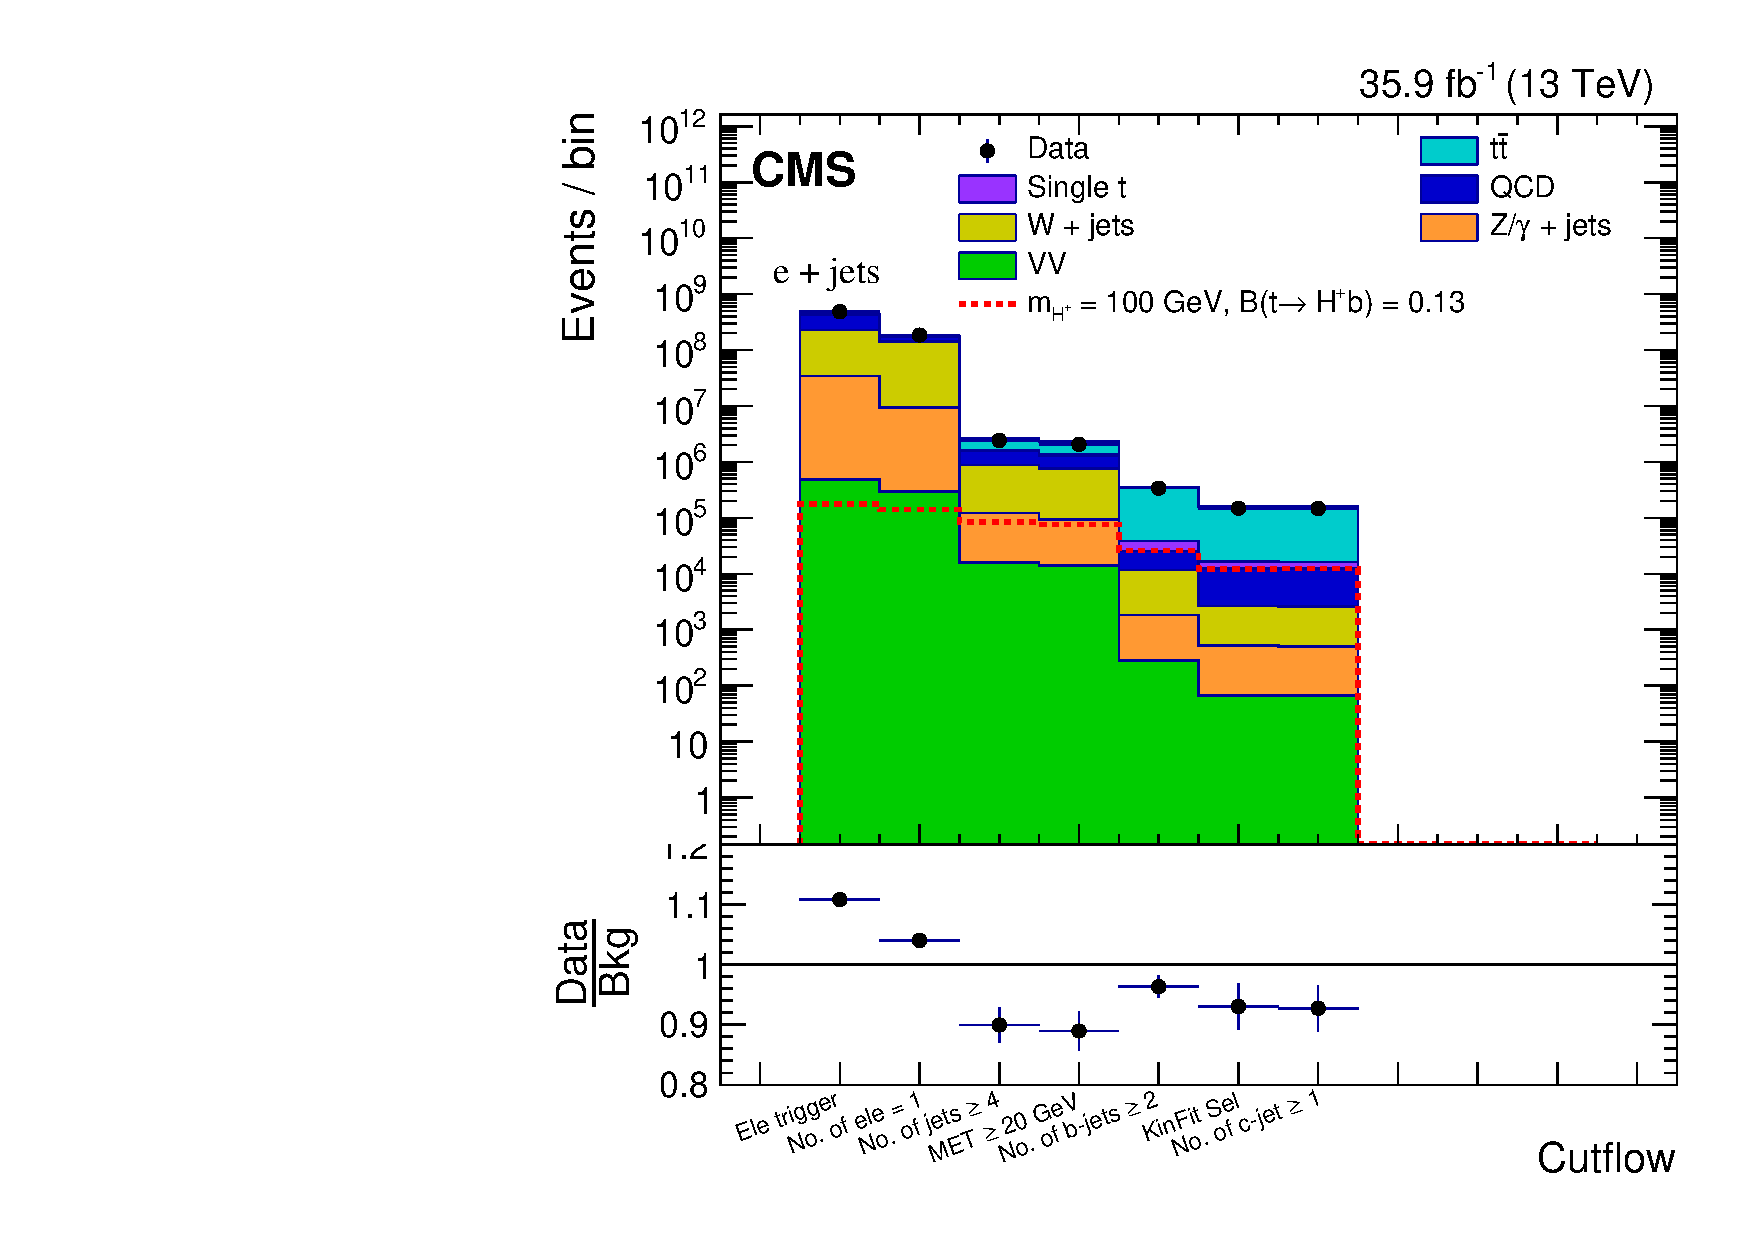
\includegraphics[width=0.50\linewidth]{Image/Electron/cutflow_ele.pdf}}
\caption{ Event yields after various selection cuts for the \mujets and \ejets channel.} 
\label{fig:cutflow}
\end{figure}

\begin{table}
    \caption{Event yields after various selection cuts for the \mujets
    channel. The $W + jets$ process is the dominant background upto 1-lepton 
    selection. When the events are required to have $N_{jets} \geq 4$, the 
    \ttjets becomes the dominant background. The QCD events are 
    from MC QCD samples as listed in Table~\ref{tab:mcSample}. The MC signal
process corresponds to $m_{H^+}=120$ GeV.}
\label{tab:cutflow_mu}
\centering

\begin{adjustbox}{max width=\textwidth}
\begin{tabular}{cccccccc}
\multicolumn{5}{c}{ } \\
\hline 
\hline 
\multicolumn{1}{ c}{Process } & \multicolumn{1}{ c}{ Trigger } & \multicolumn{1}{ c}{ $N_{muon}=1$ } &\multicolumn{1}{ c}{ $N_{jets}\ge 4$ } & \multicolumn{1}{ c}{ $\not\!\!E_T \ge 20GeV$ }&  \multicolumn{1}{ c }{ $\ge$ 2 b-jets }& \multicolumn{1}{ c}{KinFit Sel. } & \multicolumn{1}{ c}{ $\ge$1 c-jet} \\ 
\hline 
\hline 
MC signal & 232076 & 195177 & 116921 & 106839 & 35050.5 & 16932.3 & 16995.4 \\ 
\hline 
SM $t\bar{t}$ + jets & 4.02823e+06 & 2.84791e+06 & 1.4925e+06 & 1.37212e+06 & 449363 & 205678 & 204577 \\ 
Single t & 589360 & 455794 & 92348.6 & 84612 & 18402.3 & 5738.97 & 5692.71 \\ 
W + jets & 3.0976e+08 & 2.60782e+08 & 1.11136e+06 & 992060 & 13768.1 & 2979.1 & 2931.53 \\ 
$Z/\gamma$ + jets & 4.48471e+07 & 1.38263e+07 & 92247.8 & 74957.5 & 1527.75 & 440.68 & 423.088 \\ 
MC QCD & 1.44528e+08 & 4.33387e+07 & 454277 & 340874 & 14787.7 & 3159.25 & 3108.99 \\ 
VV & 653644 & 462752 & 21110.8 & 19097.7 & 515.918 & 155.957 & 156.093 \\ 
\hline 
Bkg & 5.04407e+08 & 3.21714e+08 & 3.26384e+06 & 2.88373e+06 & 498365 & 218152 & 216890 \\ 
\hline 
Data & 4.69926e+08 & 3.02859e+08 & 2.91118e+06 & 2.58404e+06 & 475120 & 203180 & 201332 \\ 
\hline 
Data/Bkg & 0.931641 & 0.941392 & 0.891948 & 0.896078 & 0.953358 & 0.931368 & 0.92827 \\ 
\hline 
\end{tabular}
\end{adjustbox}

\end{table}

\begin{table}
    \caption{Event yields after various selection cuts for the \ejets
    channel.A similar trend as that of Table~\ref{tab:cutflow_mu} is seen. The
MC signal process corresponds to $m_{H^+}=120$ GeV.}
\label{tab:cutflow_ele}
\centering

\begin{adjustbox}{max width=\textwidth}
\begin{tabular}{cccccccc}
\multicolumn{5}{c}{ } \\
\hline 
\hline 
\multicolumn{1}{ c}{Process } & \multicolumn{1}{ c}{ Trigger } & \multicolumn{1}{ c}{ $N_{ele}=1$ } &\multicolumn{1}{ c}{ $N_{jets}\ge 4$ } & \multicolumn{1}{ c}{ $\not\!\!E_T \ge 20GeV$ }&  \multicolumn{1}{ c }{ $\ge$ 2 b-jets }& \multicolumn{1}{ c}{KinFit Sel. } & \multicolumn{1}{ c}{$\ge$1 c-jet} \\ 
\hline 
\hline 
MC signal & 176707 & 142579 & 85553.5 & 77733.4 & 24927.6 & 11958.6 & 11989.3 \\ 
\hline 
SM $t\bar{t}$ + jets & 3.00506e+06 & 2.02494e+06 & 1.06093e+06 & 972693 & 313133 & 143178 & 142432 \\ 
Single t & 436965 & 312490 & 66953.2 & 61092.8 & 13159.7 & 4030.43 & 3995.41 \\ 
W + jets & 1.95738e+08 & 1.33639e+08 & 760254 & 675272 & 9814.24 & 2115.41 & 2074.13 \\ 
$Z/\gamma$ + jets & 3.38253e+07 & 9.14985e+06 & 105837 & 79926 & 1568.69 & 453.363 & 438.934 \\ 
MC QCD & 2.04408e+08 & 3.23709e+07 & 685990 & 524208 & 13850.2 & 9798.04 & 9734.67 \\ 
VV & 479876 & 297512 & 15953.1 & 14091.4 & 281.626 & 67.4654 & 67.2817 \\ 
\hline 
Bkg & 4.37893e+08 & 1.77795e+08 & 2.69591e+06 & 2.32728e+06 & 351807 & 159643 & 158742 \\ 
\hline 
Data & 4.85205e+08 & 1.84925e+08 & 2.42496e+06 & 2.07011e+06 & 338836 & 148500 & 147210 \\ 
\hline 
Data/Bkg & 1.10804 & 1.0401 & 0.899494 & 0.889495 & 0.96313 & 0.9302 & 0.927354 \\ 
\hline 
\end{tabular}
\end{adjustbox}

\end{table}

\begin{table} 
    \caption{Signal event yields for the different mass of charged Higgs after 
    various selection cuts for the \mujets channel. Event yields are almost
    same upto 1-lepton selection for all mass points. However, after the 
    $N_{jets} \geq 4$ selection (when \ttjets becomes the dominant
    background as shown in Table~\ref{tab:cutflow_mu}) the event yield for higher
    masses of the charged Higgs are reduced more compared to the lower masses. 
    The event yield reduces because of the less phase space available between 
    top-quark and charged Higgs for higher masses.}
\label{tab:cutflow_mu_sig}
\centering

\begin{adjustbox}{max width=\textwidth}
\begin{tabular}{cccccccc}
\multicolumn{5}{c}{ } \\
\hline 
\hline 
\multicolumn{1}{ c}{Process } & \multicolumn{1}{ c}{ Trigger } & \multicolumn{1}{ c}{ $N_{muon}=1$ } &\multicolumn{1}{ c}{ $N_{jets}\ge 4$ } & \multicolumn{1}{ c}{ $\not\!\!E_T \ge 20GeV$ }&  \multicolumn{1}{ c }{ $\ge$ 2 b-jets }& \multicolumn{1}{ c}{KinFit Sel. } & \multicolumn{1}{ c}{ $\ge$1 c-jet} \\ 
\hline 
\hline 
$m_{H^+}=80$ GeV & 233600 & 195175 & 112992 & 103481 & 36887.4 & 16719.5 & 16742 \\ 
$m_{H^+}=90$ GeV & 232950 & 194926 & 115096 & 105146 & 36828 & 16891.4 & 16906.2 \\ 
$m_{H^+}=100$ GeV & 233988 & 196003 & 117252 & 106948 & 37135.8 & 17547.6 & 17593.1 \\ 
$m_{H^+}=120$ GeV & 232076 & 195177 & 116921 & 106839 & 35050.5 & 16932.3 & 16995.4 \\ 
$m_{H^+}=140$ GeV & 233823 & 197826 & 111266 & 101823 & 28255.5 & 13404.1 & 13466.2 \\ 
$m_{H^+}=150$ GeV & 232614 & 197255 & 104083 & 95152 & 21645.2 & 9579.07 & 9627.62 \\ 
$m_{H^+}=155$ GeV & 233259 & 197836 & 100267 & 91809.7 & 17943.8 & 7561.99 & 7608.53 \\ 
$m_{H^+}=160$ GeV & 234566 & 199099 & 96825.5 & 88770 & 14826.9 & 5766.86 & 5790.45 \\ 
\hline 
\end{tabular}
\end{adjustbox}


\end{table}

\begin{table}
    \caption{Signal event yields for different mass of charged Higgs after 
        various selection cuts for the \ejets channel. Similar trend 
        as that of Table~\ref{tab:cutflow_mu_sig} is seen.}
\label{tab:cutflow_ele_sig}
\centering

\begin{adjustbox}{max width=\textwidth}
\begin{tabular}{cccccccc}
\multicolumn{5}{c}{ } \\
\hline 
\hline 
\multicolumn{1}{ c}{Process } & \multicolumn{1}{ c}{ Trigger } & \multicolumn{1}{ c}{ $N_{ele}=1$ } &\multicolumn{1}{ c}{ $N_{jets}\ge 4$ } & \multicolumn{1}{ c}{ $\not\!\!E_T \ge 20GeV$ }&  \multicolumn{1}{ c }{ $\ge$ 2 b-jets }& \multicolumn{1}{ c}{KinFit Sel. } & \multicolumn{1}{ c}{$\ge$1 c-jet} \\ 
\hline 
\hline 
$m_{H^+}=80$ GeV & 174714 & 140646 & 81310.9 & 74103.5 & 25873.1 & 11842 & 11850.9 \\ 
$m_{H^+}=90$ GeV & 175754 & 141375 & 83669 & 76257.2 & 26346.8 & 12196.8 & 12193 \\ 
$m_{H^+}=100$ GeV & 175150 & 140806 & 83893.1 & 76393.1 & 26123.4 & 12339.2 & 12362.7 \\ 
$m_{H^+}=120$ GeV & 176707 & 142579 & 85553.5 & 77733.4 & 24927.6 & 11958.6 & 11989.3 \\ 
$m_{H^+}=140$ GeV & 175443 & 141772 & 80110.2 & 73069.3 & 20198.9 & 9570.42 & 9618 \\ 
$m_{H^+}=150$ GeV & 177091 & 143189 & 75906.1 & 69103.3 & 15625.6 & 6948.44 & 6980.46 \\ 
$m_{H^+}=155$ GeV & 176517 & 142551 & 72361.6 & 66027.3 & 12889.3 & 5463.95 & 5497.52 \\ 
$m_{H^+}=160$ GeV & 176105 & 142405 & 70079.3 & 64024 & 10594.7 & 4224.59 & 4244.77 \\ 
\hline 
\end{tabular}
\end{adjustbox}

\end{table}
